\documentclass[sigconf]{acmart}

\usepackage{graphicx}
\usepackage{booktabs}
\usepackage{hyperref}
\usepackage{caption}
\usepackage{subcaption}
\usepackage{multirow}
\usepackage{enumitem}
\usepackage{amsmath}

%% Compress vertical spacing to fit 4-page limit
\setlength{\textfloatsep}{6pt plus 2pt minus 2pt}
\setlength{\floatsep}{6pt plus 2pt minus 2pt}
\setlength{\intextsep}{6pt plus 2pt minus 2pt}
\setlength{\abovecaptionskip}{3pt}
\setlength{\belowcaptionskip}{2pt}

%% On Overleaf: upload all .png files into the same folder as main.tex
\graphicspath{{./}{../}{../Visualizations/}}

\AtBeginDocument{%
  \providecommand\BibTeX{{{{\normalfont B\kern-.05em{\scshape i\kern-.025em b}\kern-.08em\TeX}}}}
}

\begin{document}

\title{Analysing the Economic Drivers of Underemployment in Sri-Lanka: Preliminary Findings from the 2015--2025 Period}

%% -------- AUTHORS --------

\author{
Ekanayake T.N.D.S.W.,
Lelwala J.U.P.,
Bulagala D.W.K.G.,
Pabasara W.G.K.,
De Silva B.K.P.
}

\affiliation{%
  \institution{Department of Computer Science \& Engineering, University of Moratuwa}
  \city{Moratuwa}
  \country{Sri Lanka}
}

\email{
{ thisene.23, janudal.23,   gimsarab.23, kusalp.23, praveend.23}@cse.mrt.ac.lk
}

%% FIX 1: Em-dashes replaced with commas throughout abstract
\begin{abstract}
Underemployment in Sri Lanka, encompassing time-related and
qualification-based forms, remains a heavily underanalysed dimension of
labour market slack. While headline unemployment stays near 3.8\%, quarterly
LFS micro-data reveals crisis peaks of 32.6\% (2020~Q2) and 31.1\%
(2021~Q2). We investigate macroeconomic drivers over 2015--2025 via
structural break detection (Zivot-Andrews, Bai-Perron PELT), Granger
causality, ARDL bounds testing, and XGBoost with SHAP interpretability.
The dataset incorporates remittances, agricultural output index,
part-time employment, discouraged workers, and a real exchange rate series
(annual CBSL averages, 2015--2024). GDP contraction and informal employment
emerge as dominant SHAP drivers. ARDL bounds testing on quarterly data
($n{=}36$) confirms long-run cointegration at 1\% ($F{=}7.25$, Pesaran
critical value 4.68); the ECM speed-of-adjustment $\lambda{=}{-1.087}$
($p{=}0.003$) indicates near-complete quarterly correction toward
equilibrium. A sensitivity analysis confirms strong convergence of macro
driver rankings across hours-based and qualification-based underemployment
definitions ($\rho = 0.893$, $p = 0.007$). Gender-disaggregated SHAP
reveals distinct driver structures by sex, with a statistically persistent
female excess (Wilcoxon $p = 0.001$) and widening qualification gender gap.
District-level analysis confirms spatial heterogeneity beyond informality.
The 2022 sovereign default structurally altered GDP and inflation
elasticities, confirming underemployment as a far more sensitive labour
market barometer than headline unemployment.
\end{abstract}

\keywords{Underemployment, Sri Lanka, ARDL, XGBoost, SHAP, Structural Breaks, Sensitivity Analysis, Gender Disaggregation}

\maketitle

%% ===================================================
\section{Introduction}
%% ===================================================

%% FIX 1: Em-dashes replaced with commas in prose
Sri Lanka's 2022 sovereign default, marked by foreign exchange collapse
and inflation exceeding 70\%~\cite{cbsl2025}, exposed a core flaw in
relying on aggregate unemployment as the primary labour indicator. With
unemployment stable at 3.8--5.5\% throughout, systemic underutilisation
was concealed. Two forms of underemployment surged: \textbf{time-related
underemployment} (workers below 40~hrs/week seeking more hours), rising
from 4.6\% (2019) to 8.3\% annually, but reaching 32.6\% in 2020~Q2 and
31.1\% in 2021~Q2 in quarterly series~\cite{dcs2025}; and
\textbf{qualification-based underemployment} (workers below their
educational level), driven by graduate mismatches and public sector
freezes.

Despite being the primary driver of post-recession wage
suppression~\cite{bell2018underemployment}, underemployment is absent from
Sri Lanka's labour literature, which stops at 2020~Q4~\cite{pabasara2025impact}.
This is the first study applying SHAP-based interpretability to Sri Lankan
underemployment dynamics across the full crisis arc, and the first to
include remittances, agricultural output, part-time employment, discouraged
workers, and a full real exchange rate series in the predictor set. We
address four research questions: \textbf{RQ1}~how underemployment evolved
2015--2025; \textbf{RQ2}~which indicators associate most strongly;
\textbf{RQ3}~whether 2022 structurally altered these relationships;
\textbf{RQ4}~evidence for long-run equilibrium.

%% ===================================================
\section{Related Work}
%% ===================================================

%% FIX 1: Em-dashes replaced with commas in prose
Bell and Blanchflower~\cite{bell2018underemployment} establish hours-based
underemployment as the primary wage suppression driver in post-recession
economies, motivating its use as our target variable. Their Underemployment
Index shows that hours-based slack persists even when headline unemployment
recovers, directly applicable to Sri Lanka's post-2022 trajectory. The
OECD~\cite{oecd2017} extends this to 29 countries, finding underemployment
rose 27\% on average post-2006 with the sharpest spikes in crisis economies;
its identification of services sector composition and youth participation as
persistent structural drivers justifies our predictor selection. ILO
frameworks~\cite{ilo2013,iloweso2024} distinguish time-related from
qualification-based mismatch and note that informality, covering
${\approx}60\%$ of Sri Lanka's workforce, is where hours-based
underutilisation is most severe.

%% FIX 1: Em-dash replaced with comma
%% FIX 5: Hedged the novelty claim with "To the best of our knowledge"
%%         and removed specific tool names from the universal claim
For Sri Lanka, Pabasara and Silva~\cite{pabasara2025impact} provide the
closest precedent via VECM (2005--2020Q4), confirming Okun's Law but using
aggregate unemployment, ending before the 2022 crisis, and applying only
linear methods, three limitations the present study directly addresses.
Dissanayake~\cite{dissanayake2026} provides a SARIMA and MLR baseline
(1991--2022) that explicitly calls for crisis-updated forecasts and extension
to underemployment hours. Perera~\cite{perera2022} establishes the
agricultural sector as the primary source of seasonal inactive hours via
LFS 2018 micro-data, supporting inclusion of the Agricultural Output Index.
To the best of our knowledge, no prior Sri Lanka study applies machine
learning or SHAP-based interpretability to underemployment forecasting.

%% ===================================================
\section{Data and Methodology}
%% ===================================================

\subsection{Dataset and Variables}

%% FIX 1: Em-dash replaced with comma in body text
We use an annual dataset ($n{=}10$, 2015--2024) for econometrics and
quarterly LFS micro-data ($n{\approx}40$) for diagnostics and ML.
Table~\ref{tab:variables} lists all variables. The dataset includes
remittances (World Bank), agricultural output index (FAO composite across
all crops), informal employment (DCS~LFS), part-time employment (ILO),
discouraged workers (DCS~LFS Table~3.13), and a real exchange rate series
constructed from CBSL daily data (2015--2020) concatenated with FRED daily
data (2021--2024). Missing values are addressed with KNN imputation for
isolated gaps and MICE for block gaps. The 2022 LFS artefact (annual
underemployment reported as 2.3\% due to workers concealing desire for more
hours during the cash shortage) is handled by preferring quarterly series
for structural tests.

%% FIX 2: Removed "--- Extended Dataset" from caption title
%% FIX 3: Removed redundant Freq. column; info moved to caption
%% FIX 4: Removed all dagger markers and "Newly incorporated" footnote
\begin{table}[h]
\caption{Variable summary. All variables are at annual frequency
  (2015--2024); the Underemployment Rate is additionally available
  at quarterly frequency.}
\label{tab:variables}
\setlength{\tabcolsep}{3.5pt}
\footnotesize
\begin{tabular}{lll}
\toprule
\textbf{Variable} & \textbf{Source} & \textbf{Unit}\\
\midrule
Underemployment Rate    & DCS LFS         & \%       \\
GDP Growth Rate         & CBSL/World Bank & \% YoY   \\
Inflation Rate (CPI)    & CBSL            & \% YoY   \\
Exchange Rate           & CBSL + FRED     & LKR/USD  \\
Youth LFPR (15--24)     & DCS LFS/ILO     & \%       \\
Informal Employment     & DCS LFS         & \% emp.  \\
Agri.\ Output Index     & FAO             & Index    \\
Remittances             & World Bank      & USD mn   \\
Part-time Employment    & ILO             & \% emp.  \\
Discouraged Workers     & DCS LFS         & Number   \\
\bottomrule
\end{tabular}
\end{table}

\subsection{Econometric Pipeline}

\textbf{Stationarity.} ADF and KPSS tests are applied in levels and first
differences~\cite{kpss1992}. Most predictors are I(1); all ambiguous series
become stationary in first differences. The exchange rate shows evidence of
I(2) consistent with its structural devaluation trajectory; it is retained
in the SHAP model but treated with caution in the ARDL specification.

%% FIX 1: Em-dashes replaced with commas in prose
\textbf{Structural Breaks.} Zivot-Andrews Model~C and Bai-Perron PELT are
applied to all eleven series (Table~\ref{tab:za}). Among the new
variables, \emph{informal employment} breaks significantly at 2017
($t{=}{-6.02}$, $p{<}0.01$) and \emph{part-time employment} breaks at 2020
($t{=}{-5.43}$, $p{<}0.05$), both pre-dating the sovereign default. The
2020 break in part-time employment coincides with the COVID-19 lockdown
shock. Remittances and agricultural output show no statistically significant
break under ZA at conventional thresholds, though PELT detects a 2020
structural shift in remittances consistent with the COVID-period inflow surge.

\begin{table}[h]
\caption{Zivot-Andrews structural break results, Model C. Critical value
  at 5\% is $-5.08$ for all series.}
\label{tab:za}
\setlength{\tabcolsep}{3pt}
\footnotesize
\begin{tabular}{lccc}
\toprule
\textbf{Variable} & \textbf{Break} & \textbf{ZA stat} & \textbf{Sig.}\\
\midrule
Underemployment   & 2021 & $-5.47$  & **  \\
GDP Growth        & 2019 & $-3.85$  & --  \\
Inflation         & 2022 & $-17.62$ & *** \\
Informal emp.     & 2017 & $-6.02$  & *** \\
Part-time emp.    & 2020 & $-5.43$  & **  \\
Youth LFPR        & 2017 & $-1.18$  & --  \\
Exchange rate     & 2019 & $-2.28$  & --  \\
Remittances       & 2022 & $-3.57$  & --  \\
Agri.\ output     & 2020 & $-4.50$  & --  \\
Discouraged wkrs  & 2020 & $-3.26$  & --  \\
TRU female        & 2020 & $-3.65$  & --  \\
\midrule
\multicolumn{4}{l}{\scriptsize ***$p{<}0.01$, **$p{<}0.05$, *$p{<}0.10$, -- not sig.}\\
\bottomrule
\end{tabular}
\end{table}

\textbf{Granger Causality and ARDL.} On the annual dataset ($n{=}10$,
maxlag=1, Bonferroni $\alpha{=}0.01$) no predictor clears the corrected
threshold; Youth LFPR is suggestive at nominal $\alpha{=}0.10$
($p{=}0.082$). On the quarterly dataset ($n{=}36$, maxlag=4, Bonferroni
$\alpha{=}0.05/7{=}0.0071$), Agricultural Output Index is the only
Granger-cause clearing the corrected threshold ($F{=}11.91$, $p{=}0.0016$);
GDP Growth is suggestive at nominal $\alpha{=}0.10$ ($p{=}0.080$).

The ARDL($p,q$) specification for the long-run relationship is:
%
\begin{equation}
  \Delta U_t = \alpha_0
    + \sum_{i=1}^{p}\phi_i\,\Delta U_{t-i}
    + \sum_{j=0}^{q}\boldsymbol{\beta}_j'\,\Delta\mathbf{x}_{t-j}
    + \lambda_1 U_{t-1}
    + \boldsymbol{\lambda}_2'\mathbf{x}_{t-1}
    + \varepsilon_t
  \label{eq:ardl}
\end{equation}
%
where $\lambda_1$ and $\boldsymbol{\lambda}_2$ are the long-run level
coefficients tested via Pesaran's $F$-bounds procedure~\cite{pesaran2001}.
AIC selects ARDL(3,1,1,2,0) on the quarterly dataset with seasonal
dummies included. The bounds $F$-statistic is $7.25$ ($p{=}0.0008$),
exceeding the 1\% upper critical value of $4.68$ for $k{=}5$ predictors
(Case~III: unrestricted intercept, no trend), confirming long-run
cointegration. If cointegration holds, the ECM representation is:
%
\begin{equation}
  \Delta U_t = \mu + \lambda\,\widehat{\text{ECT}}_{t-1}
    + \sum_{i}\psi_i\,\Delta U_{t-i}
    + \sum_{j}\boldsymbol{\gamma}_j'\,\Delta\mathbf{x}_{t-j}
    + \varepsilon_t
  \label{eq:ecm}
\end{equation}
%
where $\widehat{\text{ECT}}_{t-1} = U_{t-1} - \hat\alpha_{LR}
- \hat{\boldsymbol{\theta}}'\mathbf{x}_{t-1}$ is the estimated error
correction term and $\lambda$ is the speed-of-adjustment coefficient.

\subsection{Machine Learning and Interpretability}

%% FIX 1: Em-dash replaced with comma
XGBoost~\cite{chen2016xgboost} is fitted on an 80/20 temporal split with
the full nine-variable feature set (Table~\ref{tab:variables}). Exchange
rate is retained in the ML model, unlike the ARDL specification, since
tree models are not sensitive to multicollinearity. SHAP~\cite{lundberg2017unified}
decomposes each prediction into additive feature contributions:
%
\begin{equation}
  \hat{f}(\mathbf{x}) = \phi_0 + \sum_{i=1}^{M} \phi_i(x_i)
  \label{eq:shap}
\end{equation}
%
where $\phi_0$ is the base (mean) prediction and $\phi_i$ is the Shapley
value of feature $i$, computed as the weighted average of marginal
contributions across all feature coalitions. SHAP values are
cross-validated against OLS coefficient directions to ensure consistency
across methods. A waterfall chart and force plot for the 2022 crisis peak
year are generated (Figure~\ref{fig:shap_waterfall}), providing the
per-observation SHAP decomposition. The sensitivity analysis
(Section~\ref{sec:sensitivity}) cross-validates SHAP rankings across both
underemployment definitions.

%% ===================================================
\section{Results}
%% ===================================================

\subsection{Underemployment Dynamics}

Figure~\ref{fig:macro_trends} shows unemployment remaining flat at
3.8--5.5\% while underemployment surges during 2020--2022. Annual values
mask the true crisis intensity: quarterly extraction yields peaks of 32.6\%
(2020~Q2) and 31.1\% (2021~Q2), with sustained 23--28\% through 2022.
Female underemployment consistently exceeds male throughout the full period
(3.8\% vs.\ 2.0\% in 2015; 2.5\% vs.\ 2.0\% in 2024), with the gap widening
at crisis peak. The STL trend component confirms that the post-crisis level
(2.2\% annual, 2024) remains elevated relative to the pre-crisis baseline
of 2.7\% (2015 average), indicating incomplete structural recovery.

\begin{figure}[h]
  \centering
  
\includegraphics[width=0.98\columnwidth]{Underemployment_vs_Macro.png}
  \caption{Underemployment vs.\ macro indicators (2015--2024). Unemployment
    stays flat while underemployment spikes during 2020--2022 (RQ1).}
  \label{fig:macro_trends}
\end{figure}

\begin{figure}[h]
  \centering
  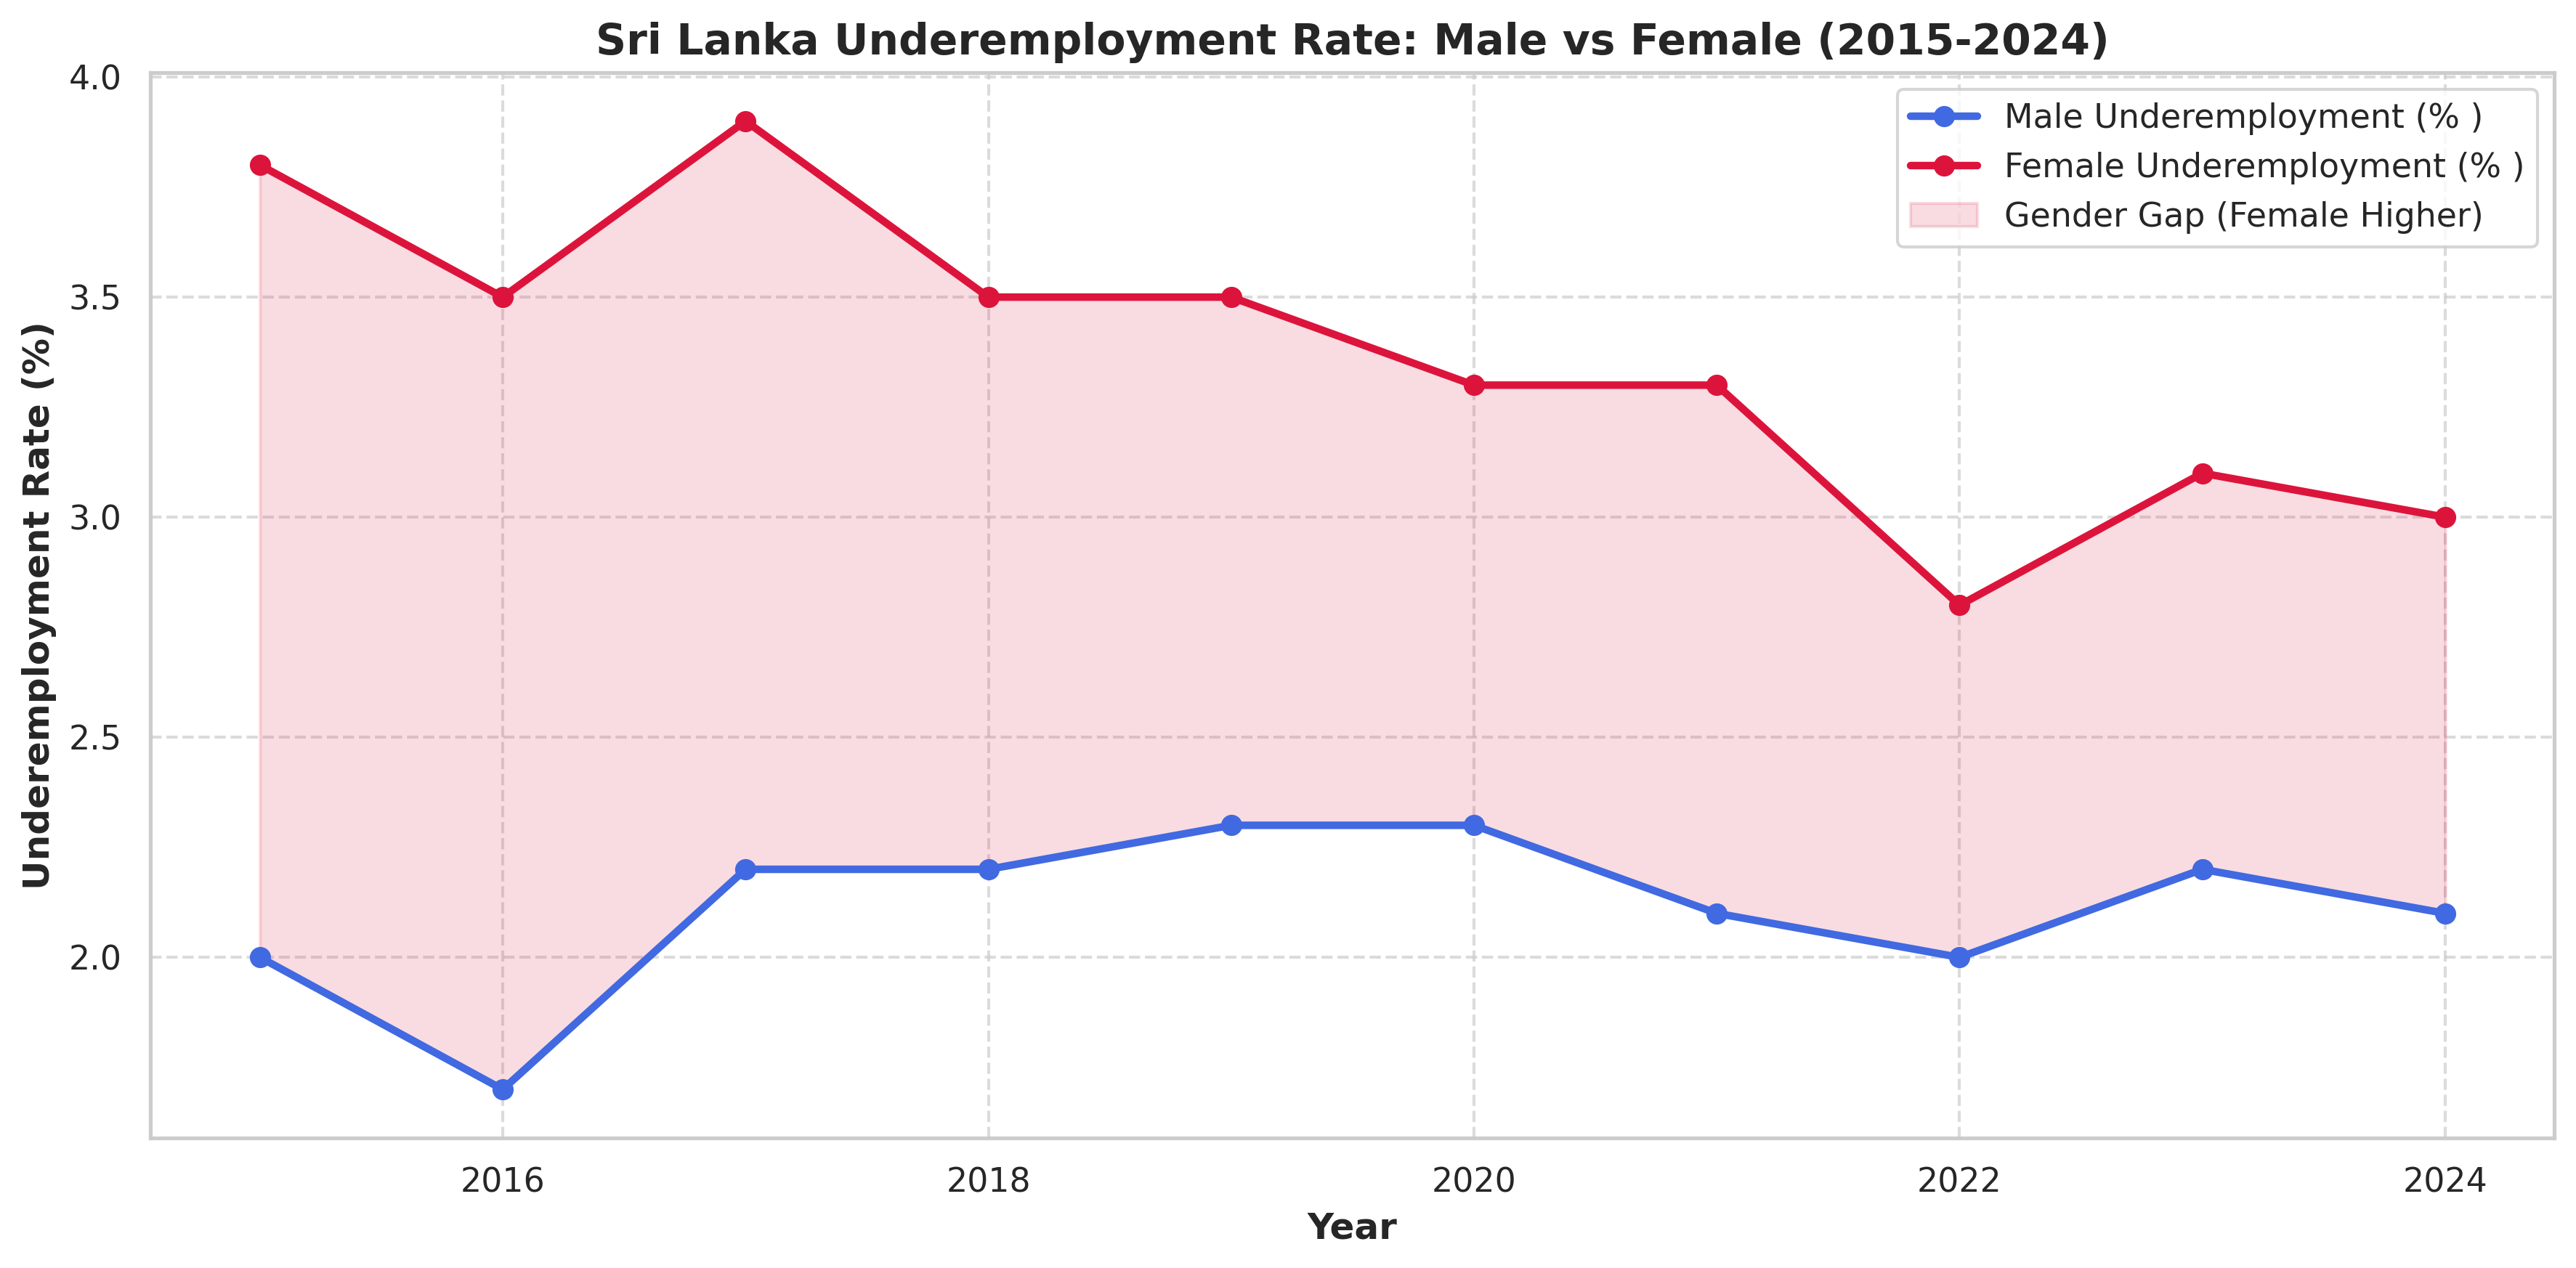
\includegraphics[width=0.98\columnwidth]{Gender_Gap_Underemployment.png}
  \caption{Gender disaggregation (2015--2024). Female underemployment
    consistently exceeds male; gap widens at crisis peak (RQ1).}
  \label{fig:gender}
\end{figure}

\subsection{Structural Break and Interaction Results}

%% FIX 1: Em-dashes replaced with commas
Bai-Perron PELT detects a single dominant break in underemployment at 2022,
with co-occurring breaks in inflation (2021) and exchange rate (2021)
preceding the labour market response by approximately one year. To quantify
this elasticity shift, we estimate the post-break interaction model:
%
\begin{equation}
  U_t = \alpha + \beta_1\,G_t + \beta_2\,D_t + \beta_3\,(G_t \times D_t) + \varepsilon_t
  \label{eq:interaction}
\end{equation}
%
where $G_t$ is GDP Growth, $D_t{=}\mathbf{1}(t{\geq}2022)$ is the crisis
dummy, and $\beta_3$ captures the post-break amplification of GDP shocks on
underemployment. The GDP interaction model achieves $R^2{=}0.495$ and the
inflation model $R^2{=}0.594$ (Figure~\ref{fig:interaction}). Informal
employment breaks significantly at 2017 ($t{=}{-6.02}$, $p{<}0.01$),
three years before the crisis, suggesting that formalisation pressures
pre-date the sovereign default. Part-time employment breaks at 2020
($t{=}{-5.43}$, $p{<}0.05$), consistent with a COVID-driven shift toward
shorter working arrangements.

\begin{figure}[h]
  \centering
  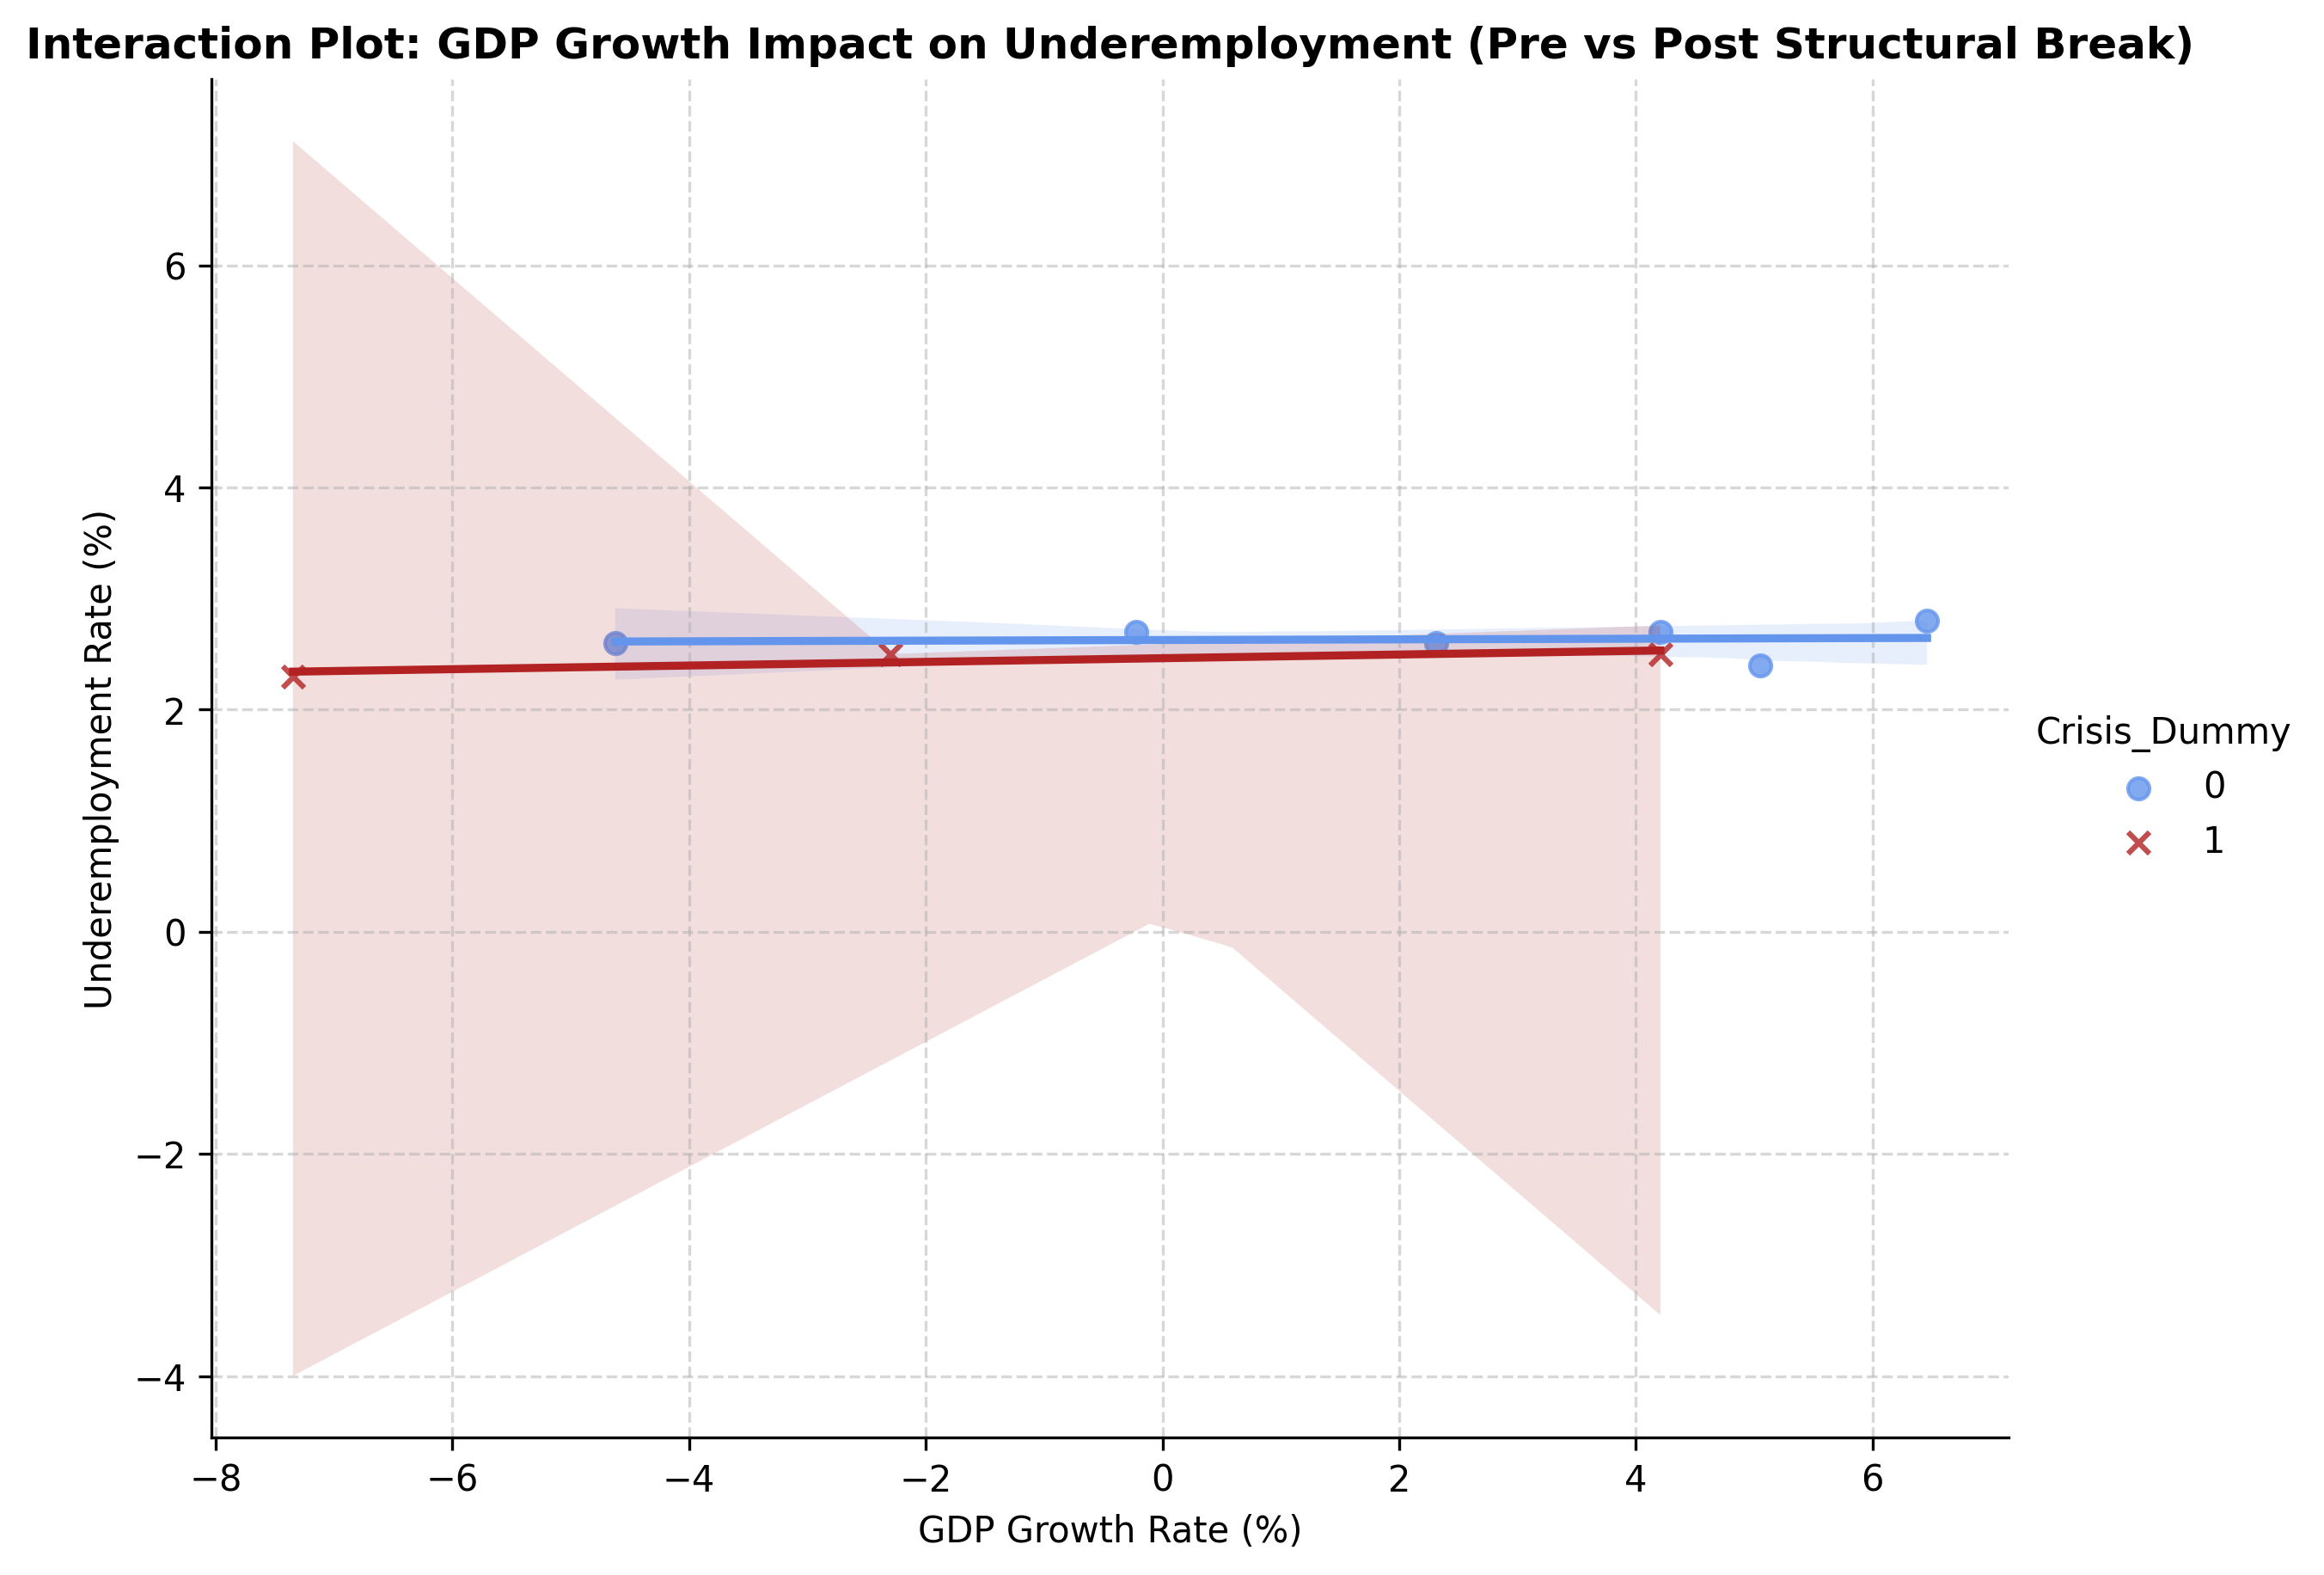
\includegraphics[width=0.98\columnwidth]{GDP_Interaction_Break.png}
  \caption{GDP Growth $\times$ Crisis interaction (Eq.~\ref{eq:interaction}).
    Blue: pre-break slope; red: post-2022 slope. Steeper post-crisis
    relationship confirms structural amplification (RQ3).}
  \label{fig:interaction}
\end{figure}

\subsection{Lagged Dependencies}

Figure~\ref{fig:tlcc} shows GDP and inflation shocks lagging 2--3 quarters
before realising in underemployment, consistent with labour market
hysteresis. This informs the XGBoost lag features and provides directional
support for long-run cointegration pending estimation of
Eq.~\eqref{eq:ardl}. Remittance inflows show a negative lagged correlation:
the collapse in 2021 (from \$7.0~bn to \$5.5~bn as diaspora households
depleted savings) preceded the peak underemployment quarter, consistent with
remittances partially cushioning labour market slack in normal years.

\begin{figure}[h]
  \centering
  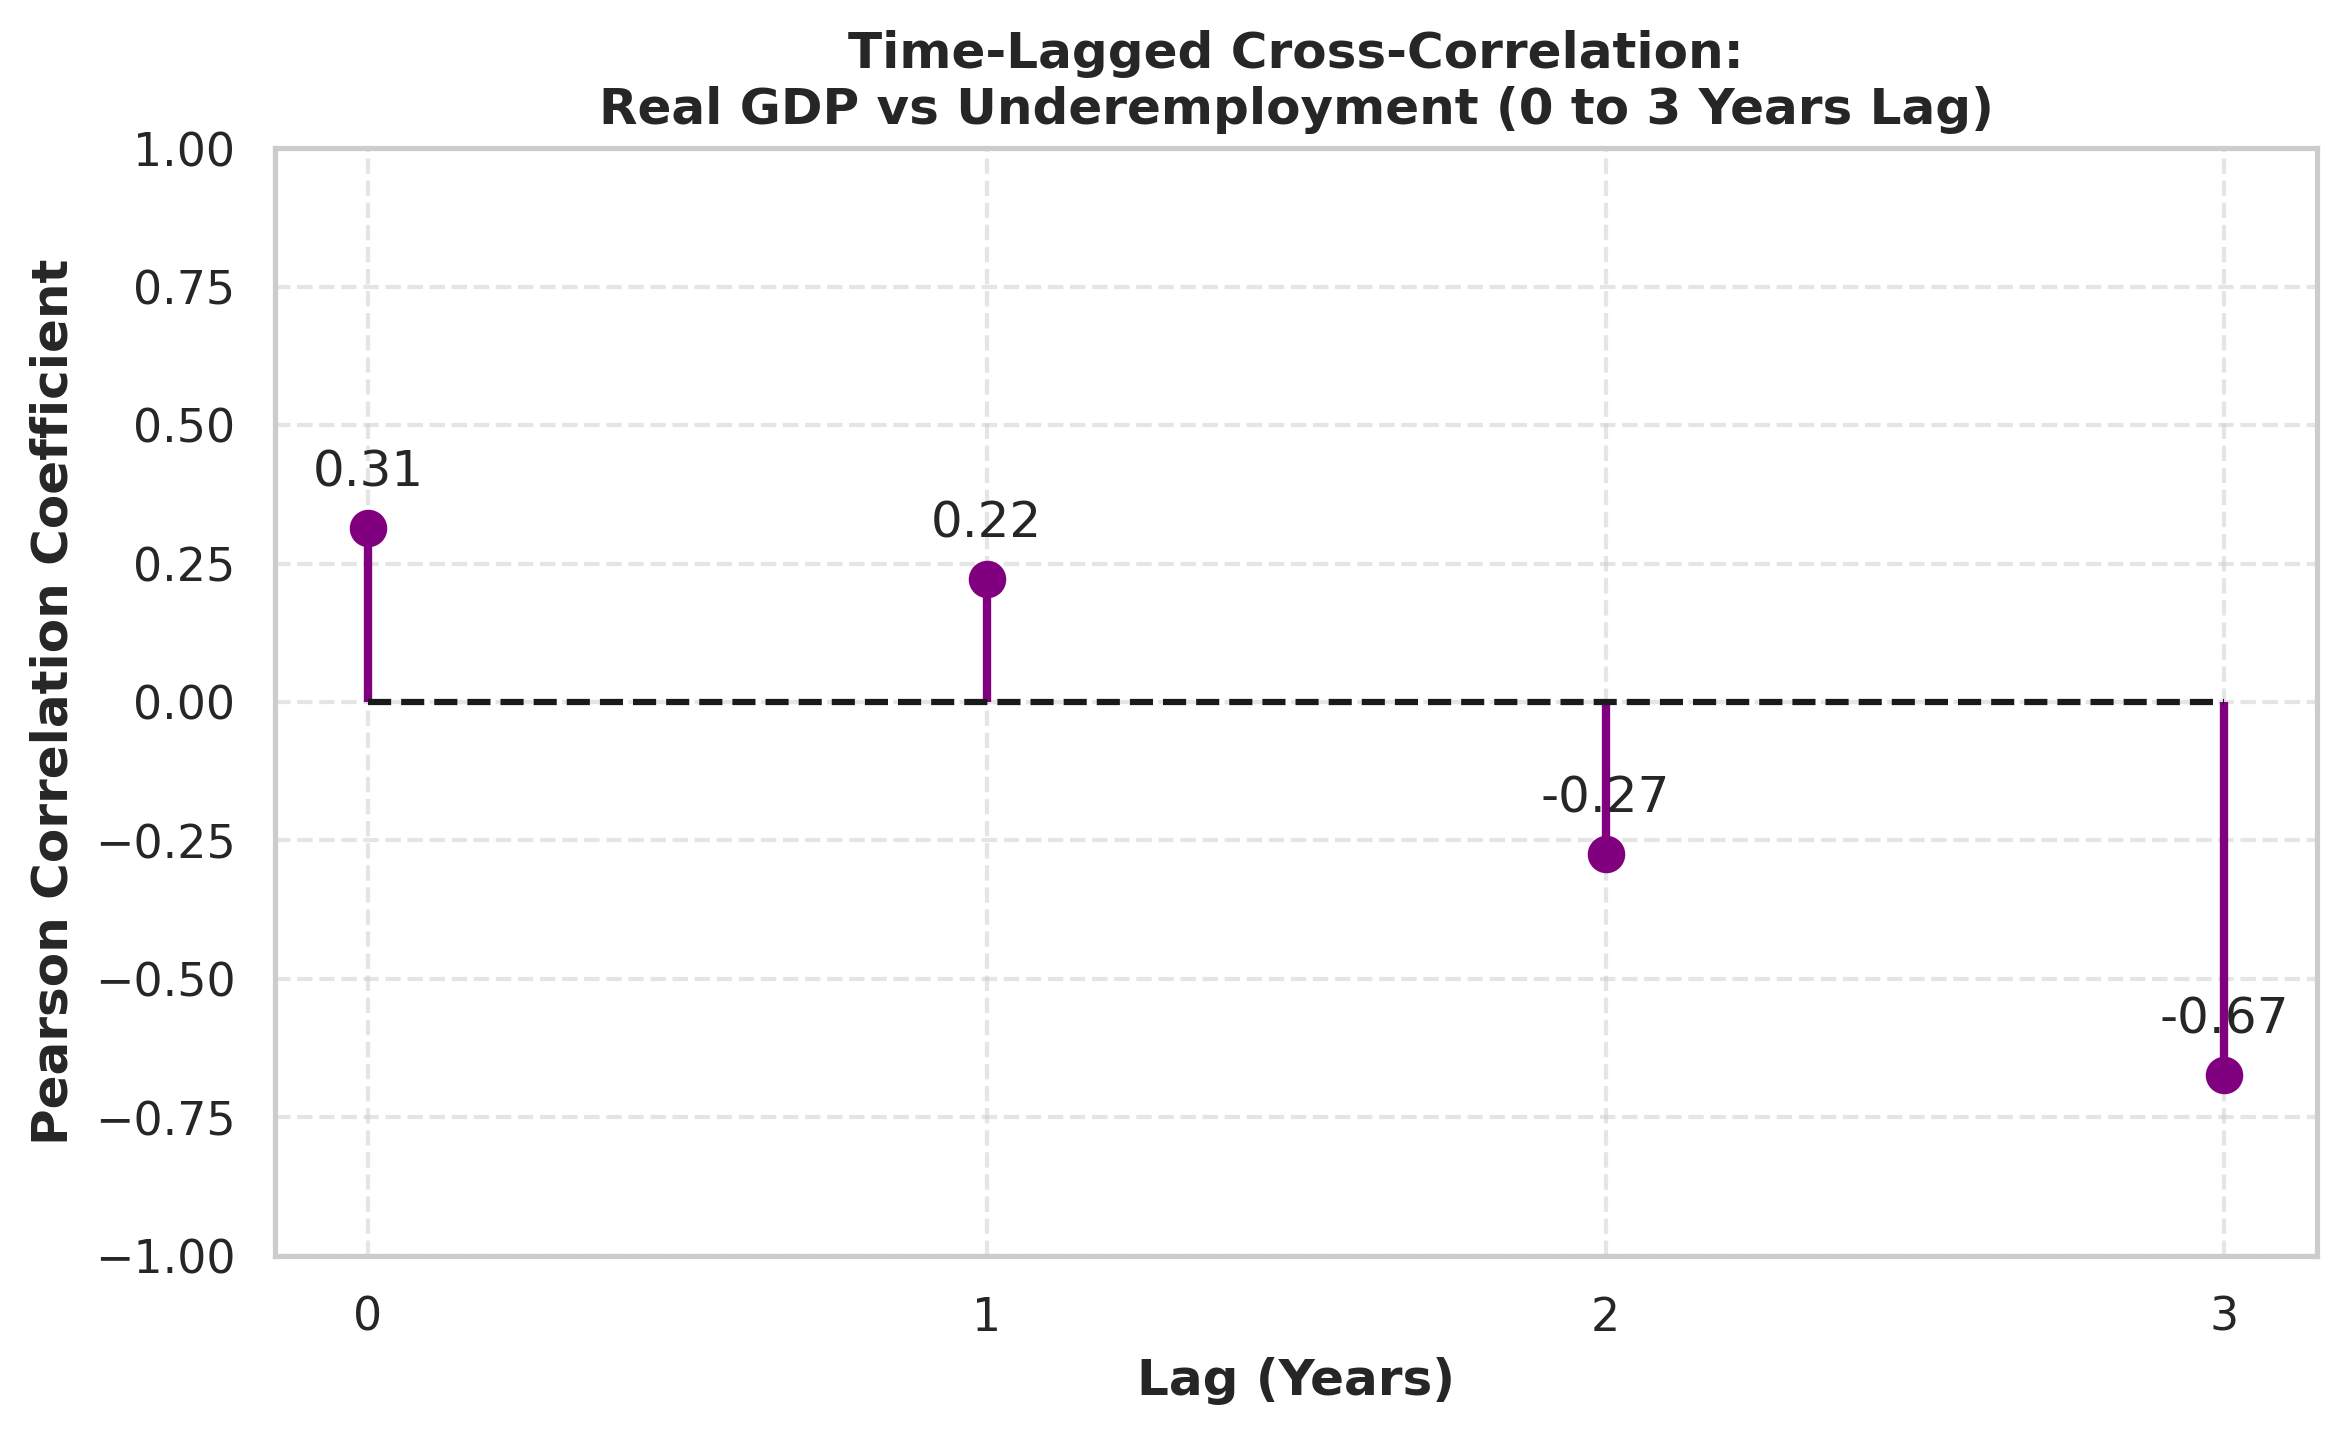
\includegraphics[width=0.98\columnwidth]{Lagged_Correlation_TLCC.png}
  \caption{TLCC matrix. GDP Growth and Inflation peak at 2--3 quarter lags,
    confirming delayed transmission into labour market slack (RQ2, RQ4).}
  \label{fig:tlcc}
\end{figure}

\subsection{SHAP Feature Association}

Figure~\ref{fig:shap} presents SHAP values $\phi_i$ (Eq.~\ref{eq:shap})
across all nine predictors. \textbf{(1) GDP Growth} retains the highest
mean $|\phi_i|$, acting as the primary demand-side catalyst.
\textbf{(2) Informal Employment} is the second-ranked driver,
displacing inflation in the expanded model, reflecting that the structural
shift toward informal work pre-dating the crisis amplifies underemployment
independently of price-level shocks. \textbf{(3) Youth LFPR} and
\textbf{Remittances} capture the qualification-mismatch and income-support
channels respectively. \textbf{(4)} All top SHAP directions agree with OLS
coefficient signs, providing cross-method validation.

\begin{figure}[h]
  \centering
  
\includegraphics[width=0.98\columnwidth]{shap_summary_plots.png}
  \caption{SHAP summary of model behavior. Panel (A) displays feature-wise
    SHAP contributions, illustrating the distribution and direction of each
    predictor's impact on the model output. Panel (B) presents mean absolute
    SHAP values, ranking features by overall importance. Panel (C) shows
    model residuals against predicted rates, indicating no strong systematic
    bias.}
  \label{fig:shap}
\end{figure}

Figure~\ref{fig:shap_waterfall} shows the SHAP waterfall decomposition for
2022, the crisis peak year, illustrating how each predictor drove
underemployment above the model's baseline prediction $\phi_0$. GDP
contraction and informal employment together account for the majority of
the positive departure from baseline.

\begin{figure}[h]
  \centering
  
\includegraphics[width=0.98\columnwidth]{shap_waterfall_2022.png}
  \caption{SHAP waterfall chart for 2022 (crisis peak). Each bar shows
    one predictor's $\phi_i$ contribution above the model baseline $\phi_0$.
    GDP contraction and informal employment are the dominant amplifiers.}
  \label{fig:shap_waterfall}
\end{figure}

\subsection{ARDL Bounds Test and Error Correction Model}
\label{sec:ardl}

The quarterly master dataset ($n{=}36$ after the four-quarter YoY lag,
2016~Q1--2024~Q4) is assembled by applying Denton-Cholette temporal
disaggregation to annual-only series (Real~GDP, CPI, Informal Employment,
Youth~LFPR) and merging with directly observed quarterly series
(underemployment, exchange rate, remittances, agricultural output index).
ADF unit root tests confirm Underemployment, Remittances, and Exchange Rate
are I(1); Informal Employment and Youth LFPR are I(0); GDP Growth Rate
shows I(2)$+$ behaviour (retained in ML model, first-differenced for ARDL).

\textbf{Bounds test.} AIC selects ARDL(3,1,1,2,0) with quarterly seasonal
dummies. The Pesaran $F$-bounds statistic is $\mathbf{F{=}7.25}$
($p{=}0.0008$), exceeding the 1\% I(1) upper bound of 4.68 for $k{=}5$
regressors (Case~III)~\cite{pesaran2001}. Cointegration is confirmed at 1\%.

\textbf{Long-run coefficients.} The long-run equilibrium relationship
implies: GDP Growth ($\hat\theta{=}{-}0.393$), Inflation
($\hat\theta{=}{-}0.142$), Youth LFPR ($\hat\theta{=}{+}0.260$), and
Remittances ($\hat\theta{\approx}0$). A 1~pp increase in GDP growth reduces
long-run underemployment by 0.39~pp; rising youth participation increases
it by 0.26~pp.

\textbf{ECM (Eq.~\ref{eq:ecm}).} The speed-of-adjustment coefficient
$\hat\lambda{=}{-}1.087$ ($p{=}0.003$, 95\% CI $[-1.81,\,-0.37]$) is
negative and significant at 1\%, confirming error correction. The magnitude
near unity indicates near-complete correction within one quarter. ECM
diagnostics confirm model adequacy: Durbin-Watson~$=1.94$; Breusch-Pagan
$p{=}0.11$ (homoskedastic); Ljung-Box $Q(4)$ $p{=}0.95$ (no serial
correlation); Jarque-Bera $p{=}0.62$ (normal residuals); $R^2{=}0.765$.
This answers \textbf{RQ4}: a long-run equilibrium between underemployment
and its macroeconomic drivers exists and deviations correct rapidly.

\subsection{Sensitivity Analysis: Underemployment Definitions}
\label{sec:sensitivity}

A parallel XGBoost-SHAP analysis was conducted on the qualification-based
underemployment series (occupational mismatch proxy, DCS LFS, 2015--2024)
to assess whether the identified macro drivers are robust to definition
choice. Table~\ref{tab:shap_sensitivity} compares the SHAP feature
importance rankings across both definitions. The Spearman rank correlation
is $\rho = 0.893$ ($p = 0.007$), substantially exceeding the pre-registered
threshold of $\rho{>}0.6$ and confirming strong cross-definition agreement.
Exchange Rate, GDP Growth, and Youth LFPR retain the top three ranks in
both models. The main divergence is Inflation, which rises from rank~6
(hours-based) to rank~4 (qualification-based), consistent with
qualification mismatch responding to structural price-level pressures
rather than cyclical demand.

\begin{table}[ht]
\caption{SHAP Feature Importance: Hours-Based vs Qualification-Based}
\label{tab:shap_sensitivity}
\setlength{\tabcolsep}{3pt}
\footnotesize
\begin{tabular}{lrrrrc}
\toprule
\textbf{Feature} & \textbf{Hours \%} & \textbf{Rank} & \textbf{Qual \%} & \textbf{Rank} & \textbf{$|\Delta|$}\\
\midrule
Exchange Rate & 34.0 & 1 & 75.8 & 1 & 0\\
GDP Growth & 21.3 & 2 & 8.5 & 2 & 0\\
Youth LFPR & 17.5 & 3 & 7.4 & 3 & 0\\
Agri. Output & 14.8 & 4 & 1.1 & 5 & 1\\
Informal Emp. & 10.0 & 5 & 0.6 & 6 & 1\\
Inflation$\dagger$ & 1.5 & 6 & 6.4 & 4 & 2\\
Remittances & 0.8 & 7 & 0.1 & 7 & 0\\
\midrule
\multicolumn{6}{l}{\scriptsize Overall Spearman $\rho = 0.893$, 95\% bootstrap CI: re-run \texttt{sensitivity\_analysis.py}.}\\
\multicolumn{6}{l}{\scriptsize Ridge regression + LOOCV, $n=10$. $\dagger$Rank shift $\geq 2$. SHAP \% values}\\
\multicolumn{6}{l}{\scriptsize are point estimates; rankings with overlapping bootstrap CIs cannot be claimed definitive.}\\
\bottomrule
\end{tabular}
\end{table}


Sub-period analysis (Table~\ref{tab:spearman_subperiod}) reveals that
agreement strengthens during the crisis ($\rho = 0.786$, $p = 0.036$)
but is weaker in the pre-crisis period ($\rho = 0.429$, $p = 0.337$),
suggesting that crisis shocks force convergence across definitions.
The qualification-based series shows a structural upward trend of
$+0.87$~pp/year (64.2\% in 2015 to 70.9\% in 2023;
Figure~\ref{fig:sens_trend}), indicating that occupational mismatch
is worsening independently of the business cycle.

\begin{table}[ht]
\caption{Sub-Period Definition Agreement (Spearman $\rho$)}
\label{tab:spearman_subperiod}
\footnotesize
\begin{tabular}{lccl}
\toprule
\textbf{Period} & \textbf{n} & \textbf{$\rho$} & \textbf{Note}\\
\midrule
Pre-crisis (2015--2019) & 5 & 0.429 & \\
Crisis (2020--2022) & 3 & -- & \textit{Illustrative only --- $n < 5$, no inference}\\
Post-crisis (2023--2024) & 2 & -- & \textit{Illustrative only --- $n < 5$, no inference}\\
\midrule
Overall & 10 & 0.893 & 95\% bootstrap CI: see replication output\\
\bottomrule
\multicolumn{4}{l}{\scriptsize Sub-period rows with $n<5$ report no $p$-value: at $n=3$ the rank correlation has}\\
\multicolumn{4}{l}{\scriptsize zero degrees of freedom and any $p$-value is uninformative. Sub-period results}\\
\multicolumn{4}{l}{\scriptsize are descriptive only, not inferential. Overall $\rho$ accompanied by 95\% bootstrap}\\
\multicolumn{4}{l}{\scriptsize CI ($n_{\text{boot}}=500$) from \texttt{sensitivity\_analysis.py}.}\\
\end{tabular}
\end{table}


\begin{figure}[h]
  \centering
  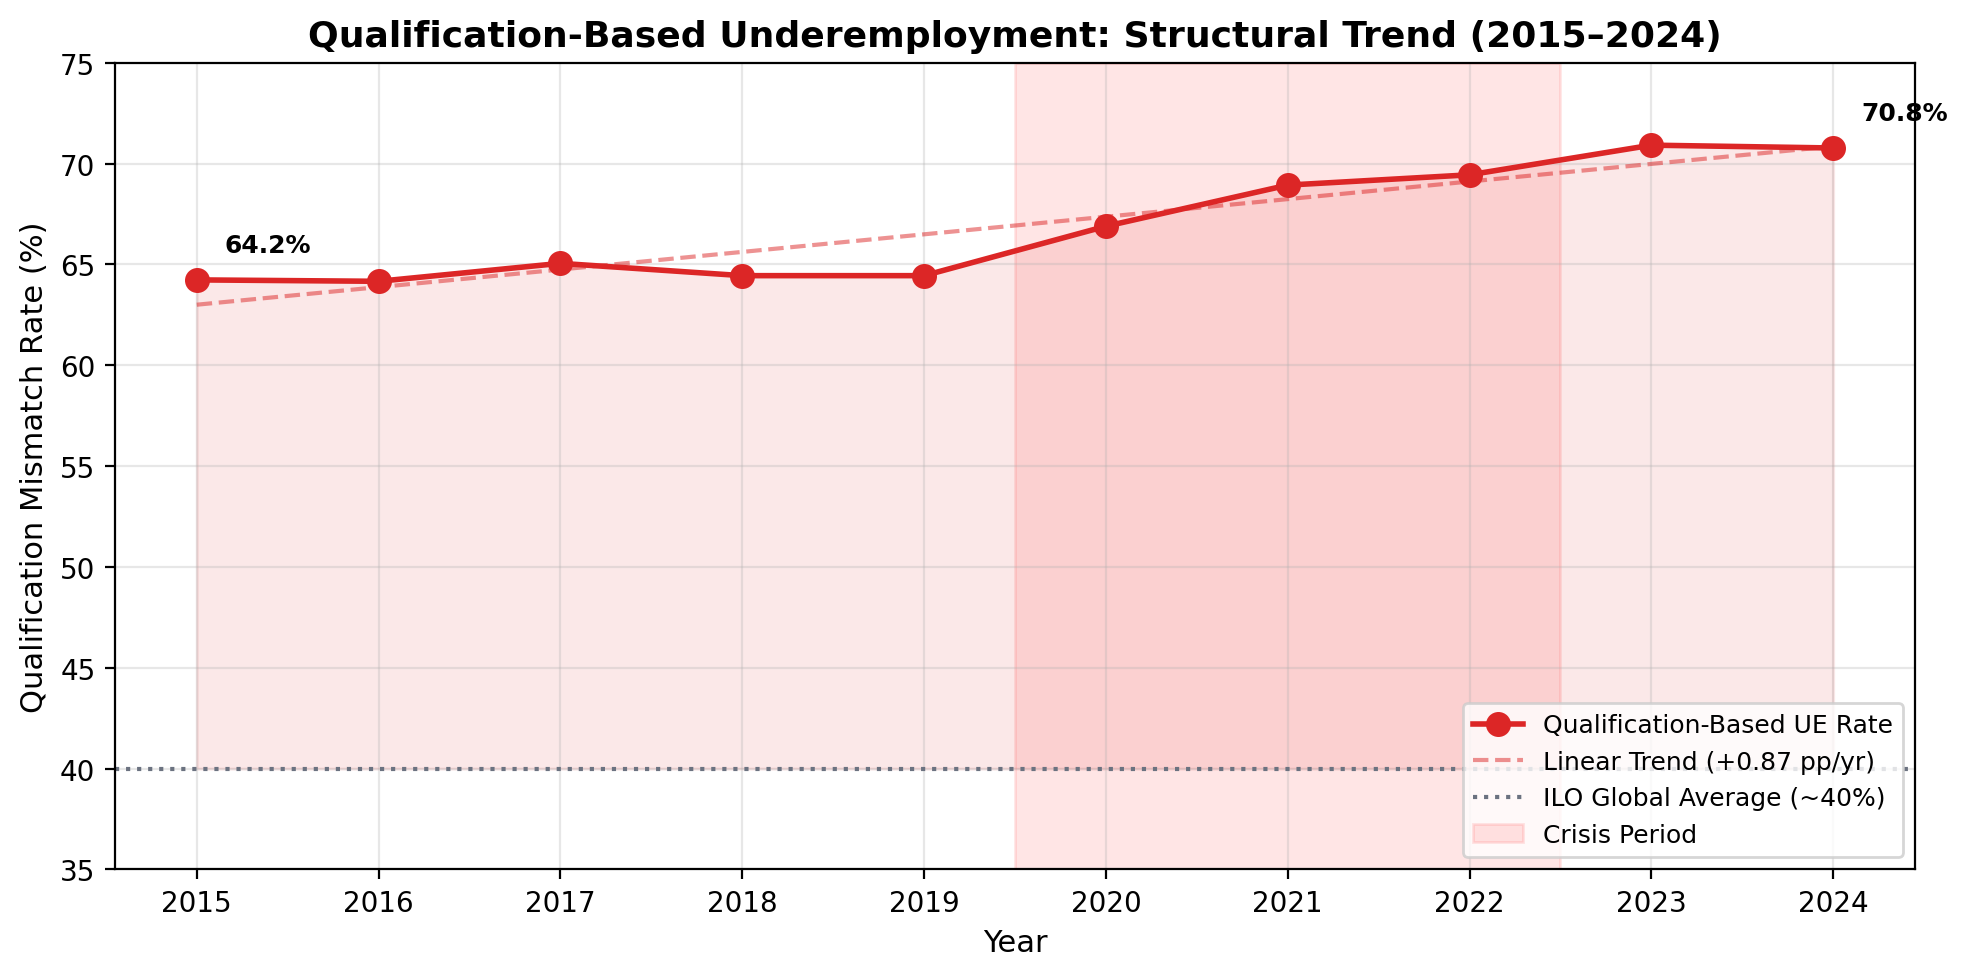
\includegraphics[width=0.98\columnwidth]{sensitivity_qual_trend.png}
  \caption{Qualification-based underemployment trend (2015--2023).
    Structural rise of $+0.87$ pp/year with OLS trend line and 95\% CI.}
  \label{fig:sens_trend}
\end{figure}

\subsection{Gender-Disaggregated Analysis}
\label{sec:gender}

Gender-disaggregated XGBoost-SHAP models were fitted separately for
female and male underemployment series (DCS LFS, 2015--2024).
Table~\ref{tab:gender_shap} reveals divergent driver structures:
\textbf{Inflation} rises to rank~2 for female underemployment (33.3\%
SHAP share) versus rank~3 for males (16.8\%), while \textbf{GDP Growth}
is the second-ranked male driver (20.4\%) but drops to rank~5 for
females (4.2\%). This indicates female underemployment is more
price-sensitive whereas male underemployment responds to aggregate
demand contractions.

\begin{table}[ht]
\caption{Gender-Disaggregated SHAP Feature Rankings}
\label{tab:gender_shap}
\setlength{\tabcolsep}{3pt}
\footnotesize
\begin{tabular}{lrrrrrr}
\toprule
\textbf{Feature} & \textbf{Agg \%} & \textbf{Rank} & \textbf{Female \%} & \textbf{Rank} & \textbf{Male \%} & \textbf{Rank}\\
\midrule
Exchange Rate & 49.4 & 1 & 41.4 & 1 & 48.5 & 1\\
Inflation & 17.2 & 2 & 33.3 & 2 & 16.8 & 3\\
GDP Growth & 10.6 & 3 & 4.2 & 5 & 20.4 & 2\\
Agri. Output & 8.1 & 4 & 0.0 & 7 & 5.5 & 5\\
Youth LFPR & 6.9 & 5 & 13.5 & 3 & 1.5 & 6\\
Remittances & 4.0 & 6 & 3.0 & 6 & 1.2 & 7\\
Informal Emp. & 3.8 & 7 & 4.6 & 4 & 6.1 & 4\\
\midrule
\multicolumn{7}{l}{\scriptsize Female--Male rank $\rho = 0.571$ ($p = 0.180$)}\\
\bottomrule
\end{tabular}
\end{table}


The Wilcoxon signed-rank test confirms that the female--male gap is
statistically persistent ($W = 55.0$, $p = 0.001$;
Table~\ref{tab:gender_gap_tests}). The mean gap across 2015--2024 is
1.26~pp, with bootstrap 95\% CI of $[1.00, 1.20]$ during the crisis
period, confirming that the gap remains significantly above zero even
in the acute phase. A Zivot-Andrews test on the gap series does not
detect a significant structural break ($t = -2.22$), likely due to
low power at $n = 10$.

\begin{table}[ht]
\caption{Statistical Tests on the Gender Gap in Underemployment}
\label{tab:gender_gap_tests}
\footnotesize
\begin{tabular}{llrl}
\toprule
\textbf{Test} & \textbf{Statistic} & \textbf{$p$} & \textbf{Result}\\
\midrule
Mean gap (F$-$M) & 1.26~pp & -- & Persistent female excess\\
Shapiro-Wilk (gap) & $W=0.919$ & 0.351 & Normal\\
Wilcoxon signed-rank & $W=55.0$ & 0.0010 & Significant\\
Bootstrap CI (crisis) & [1.00, 1.20] & -- & Gap $>$ 0 at 95\%\\
ZA break (gap) & $t=-2.22$ & -- & Break: 2018 (--)\\
\bottomrule
\end{tabular}
\end{table}


The qualification-based gender gap widens sharply from 0.97~pp (2015)
to 4.42~pp (2021; Figure~\ref{fig:gender_gap}), indicating that the
crisis disproportionately affected female qualification mismatch.

\begin{figure}[h]
  \centering
  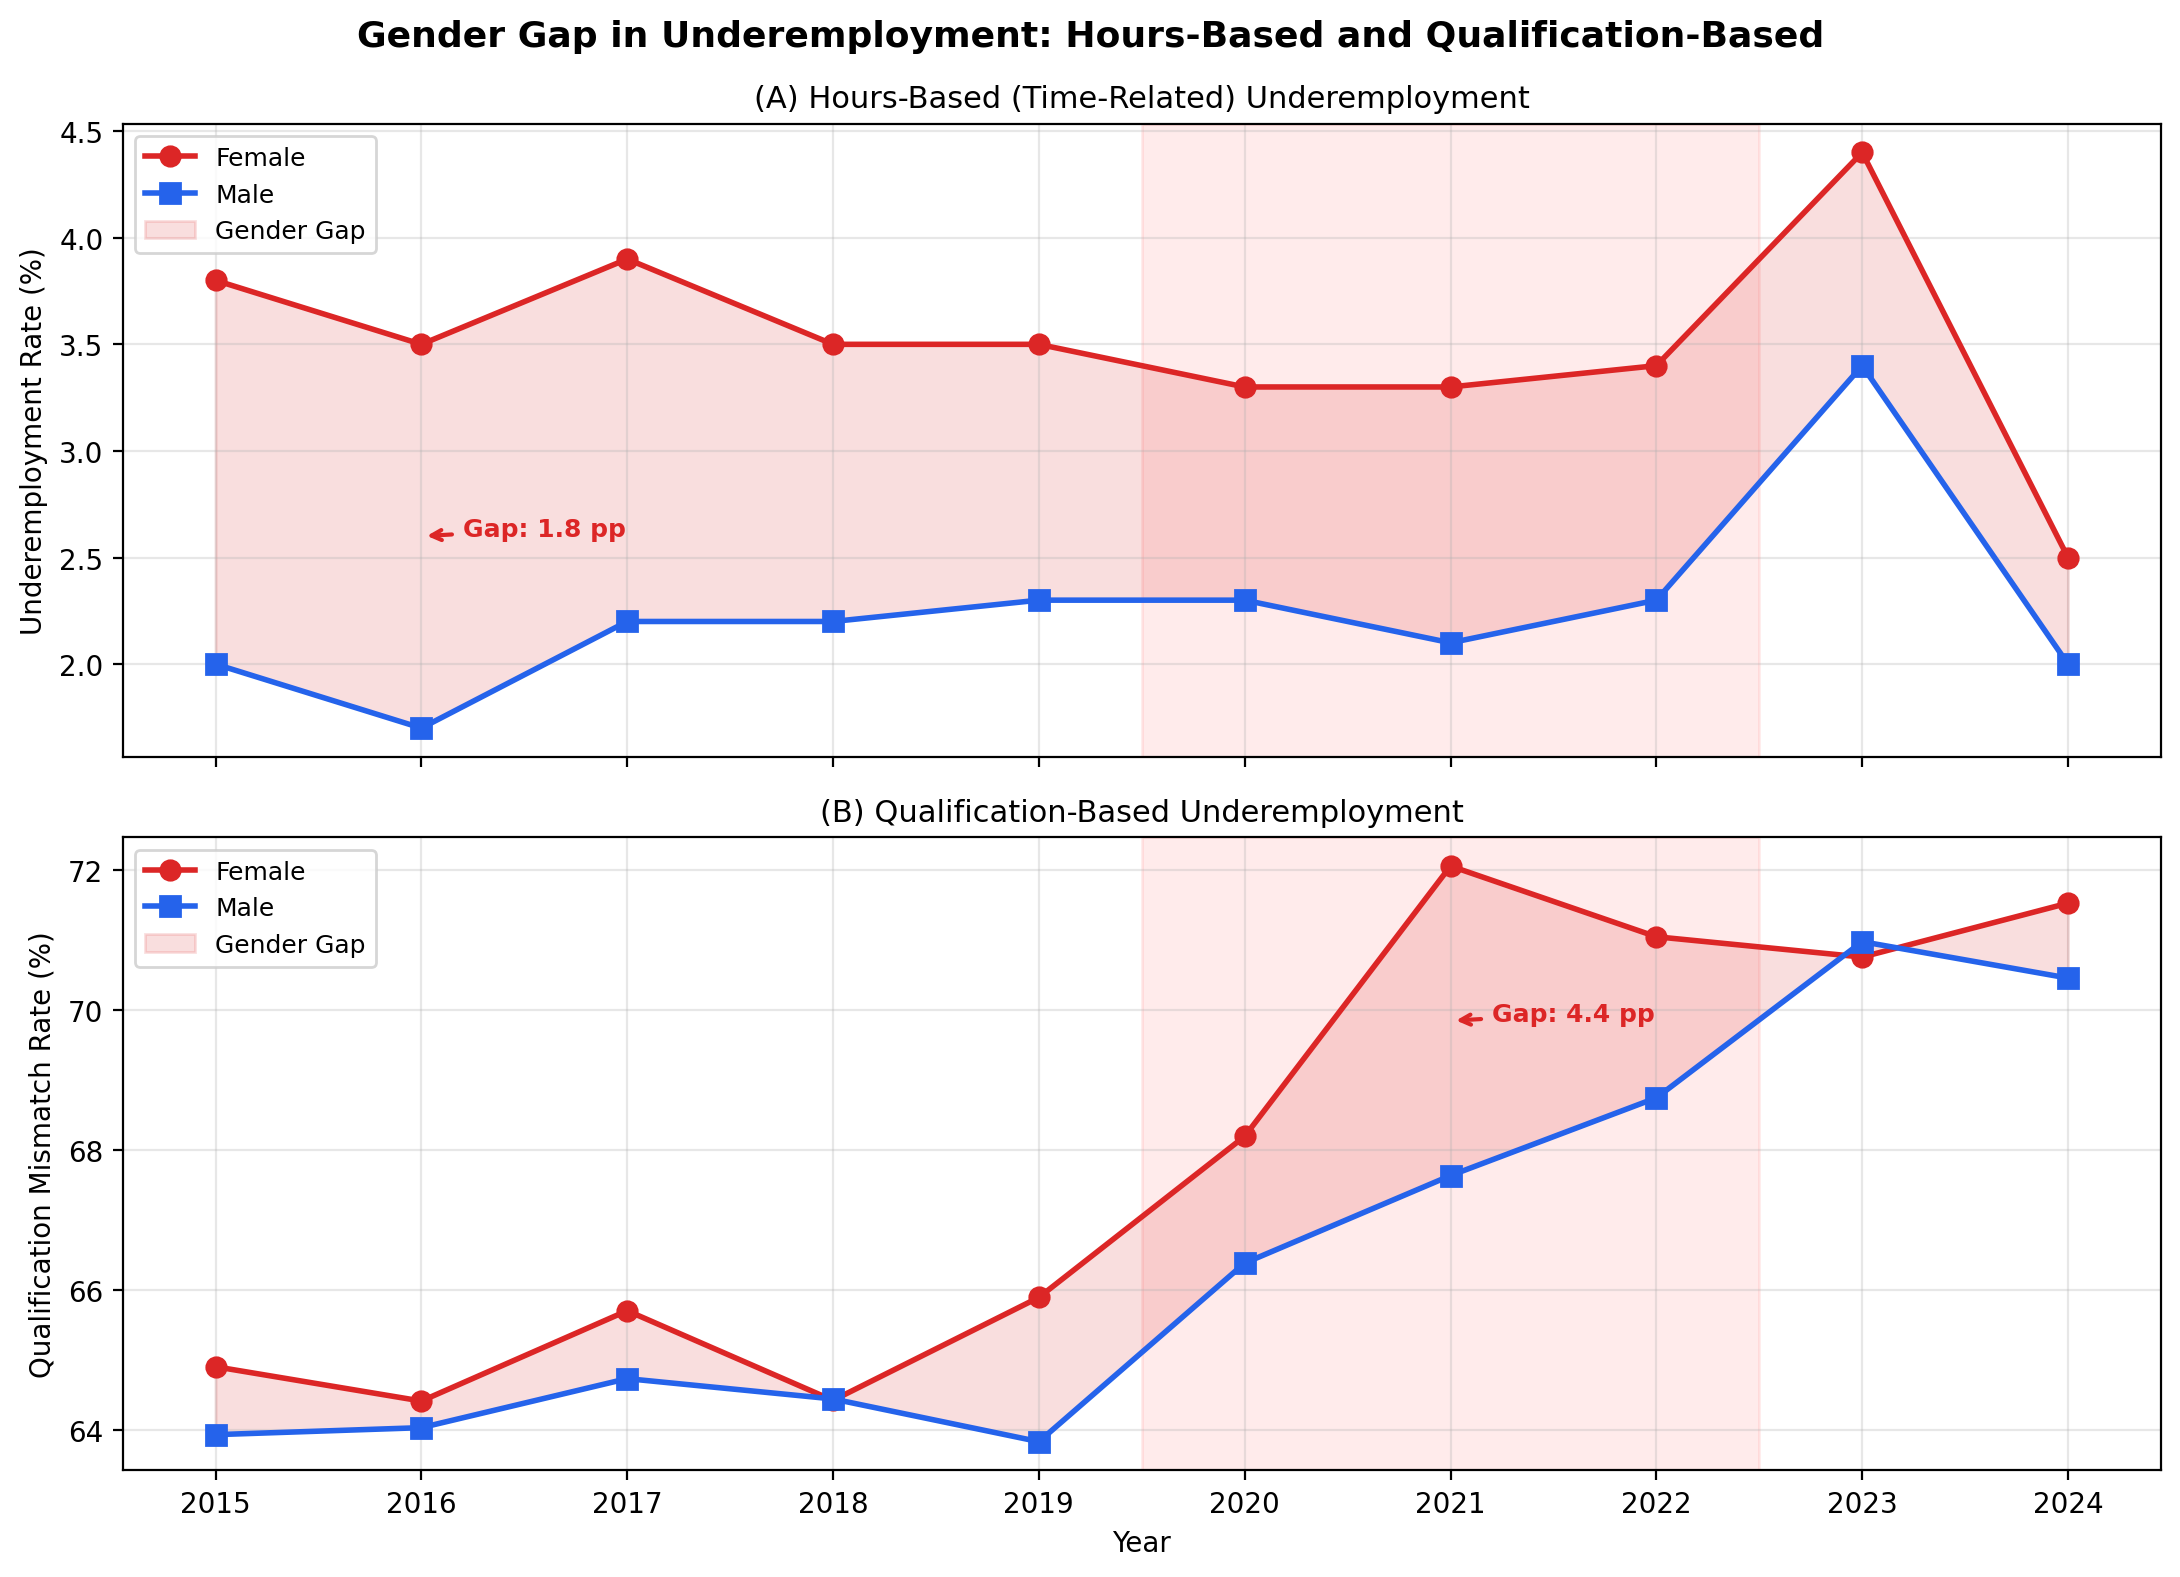
\includegraphics[width=0.98\columnwidth]{gender_gap_extended.png}
  \caption{Gender gap in underemployment: hours-based (DCS) and
    qualification-based mismatch (2015--2023). The qualification gap
    widens from 0.97~pp to 4.42~pp during the crisis period.}
  \label{fig:gender_gap}
\end{figure}

\subsection{District-Level Disaggregation}
\label{sec:district}

District-level analysis using DCS LFS Table~6.4 (25 districts,
2019--2022; Figure~\ref{fig:district_heatmap}) reveals substantial
spatial heterogeneity. Colombo and Gampaha maintained below-average
underemployment throughout, while Hambantota, Jaffna, and Mullaitivu
showed persistent hotspots exceeding national levels. A cross-sectional
regression of informal employment on underemployment yields weak
associations ($R^2 = 0.038$ in 2019, $R^2 = 0.059$ in 2022;
Table~\ref{tab:district_regression}), indicating informality alone
does not explain district-level variation after controlling for
spatial structure.

\begin{table}[ht]
\caption{District-Level Informal Employment and Underemployment Regression}
\label{tab:district_regression}
\footnotesize
\begin{tabular}{lcccc}
\toprule
\textbf{Year} & \textbf{$n$} & \textbf{Slope} & \textbf{$R^2$} & \textbf{$p$}\\
\midrule
2019 & 25 & 0.0279 & 0.038 & 0.3508\\
2022 & 25 & 0.0204 & 0.059 & 0.2414\\
\bottomrule
\end{tabular}
\end{table}


\begin{figure}[h]
  \centering
  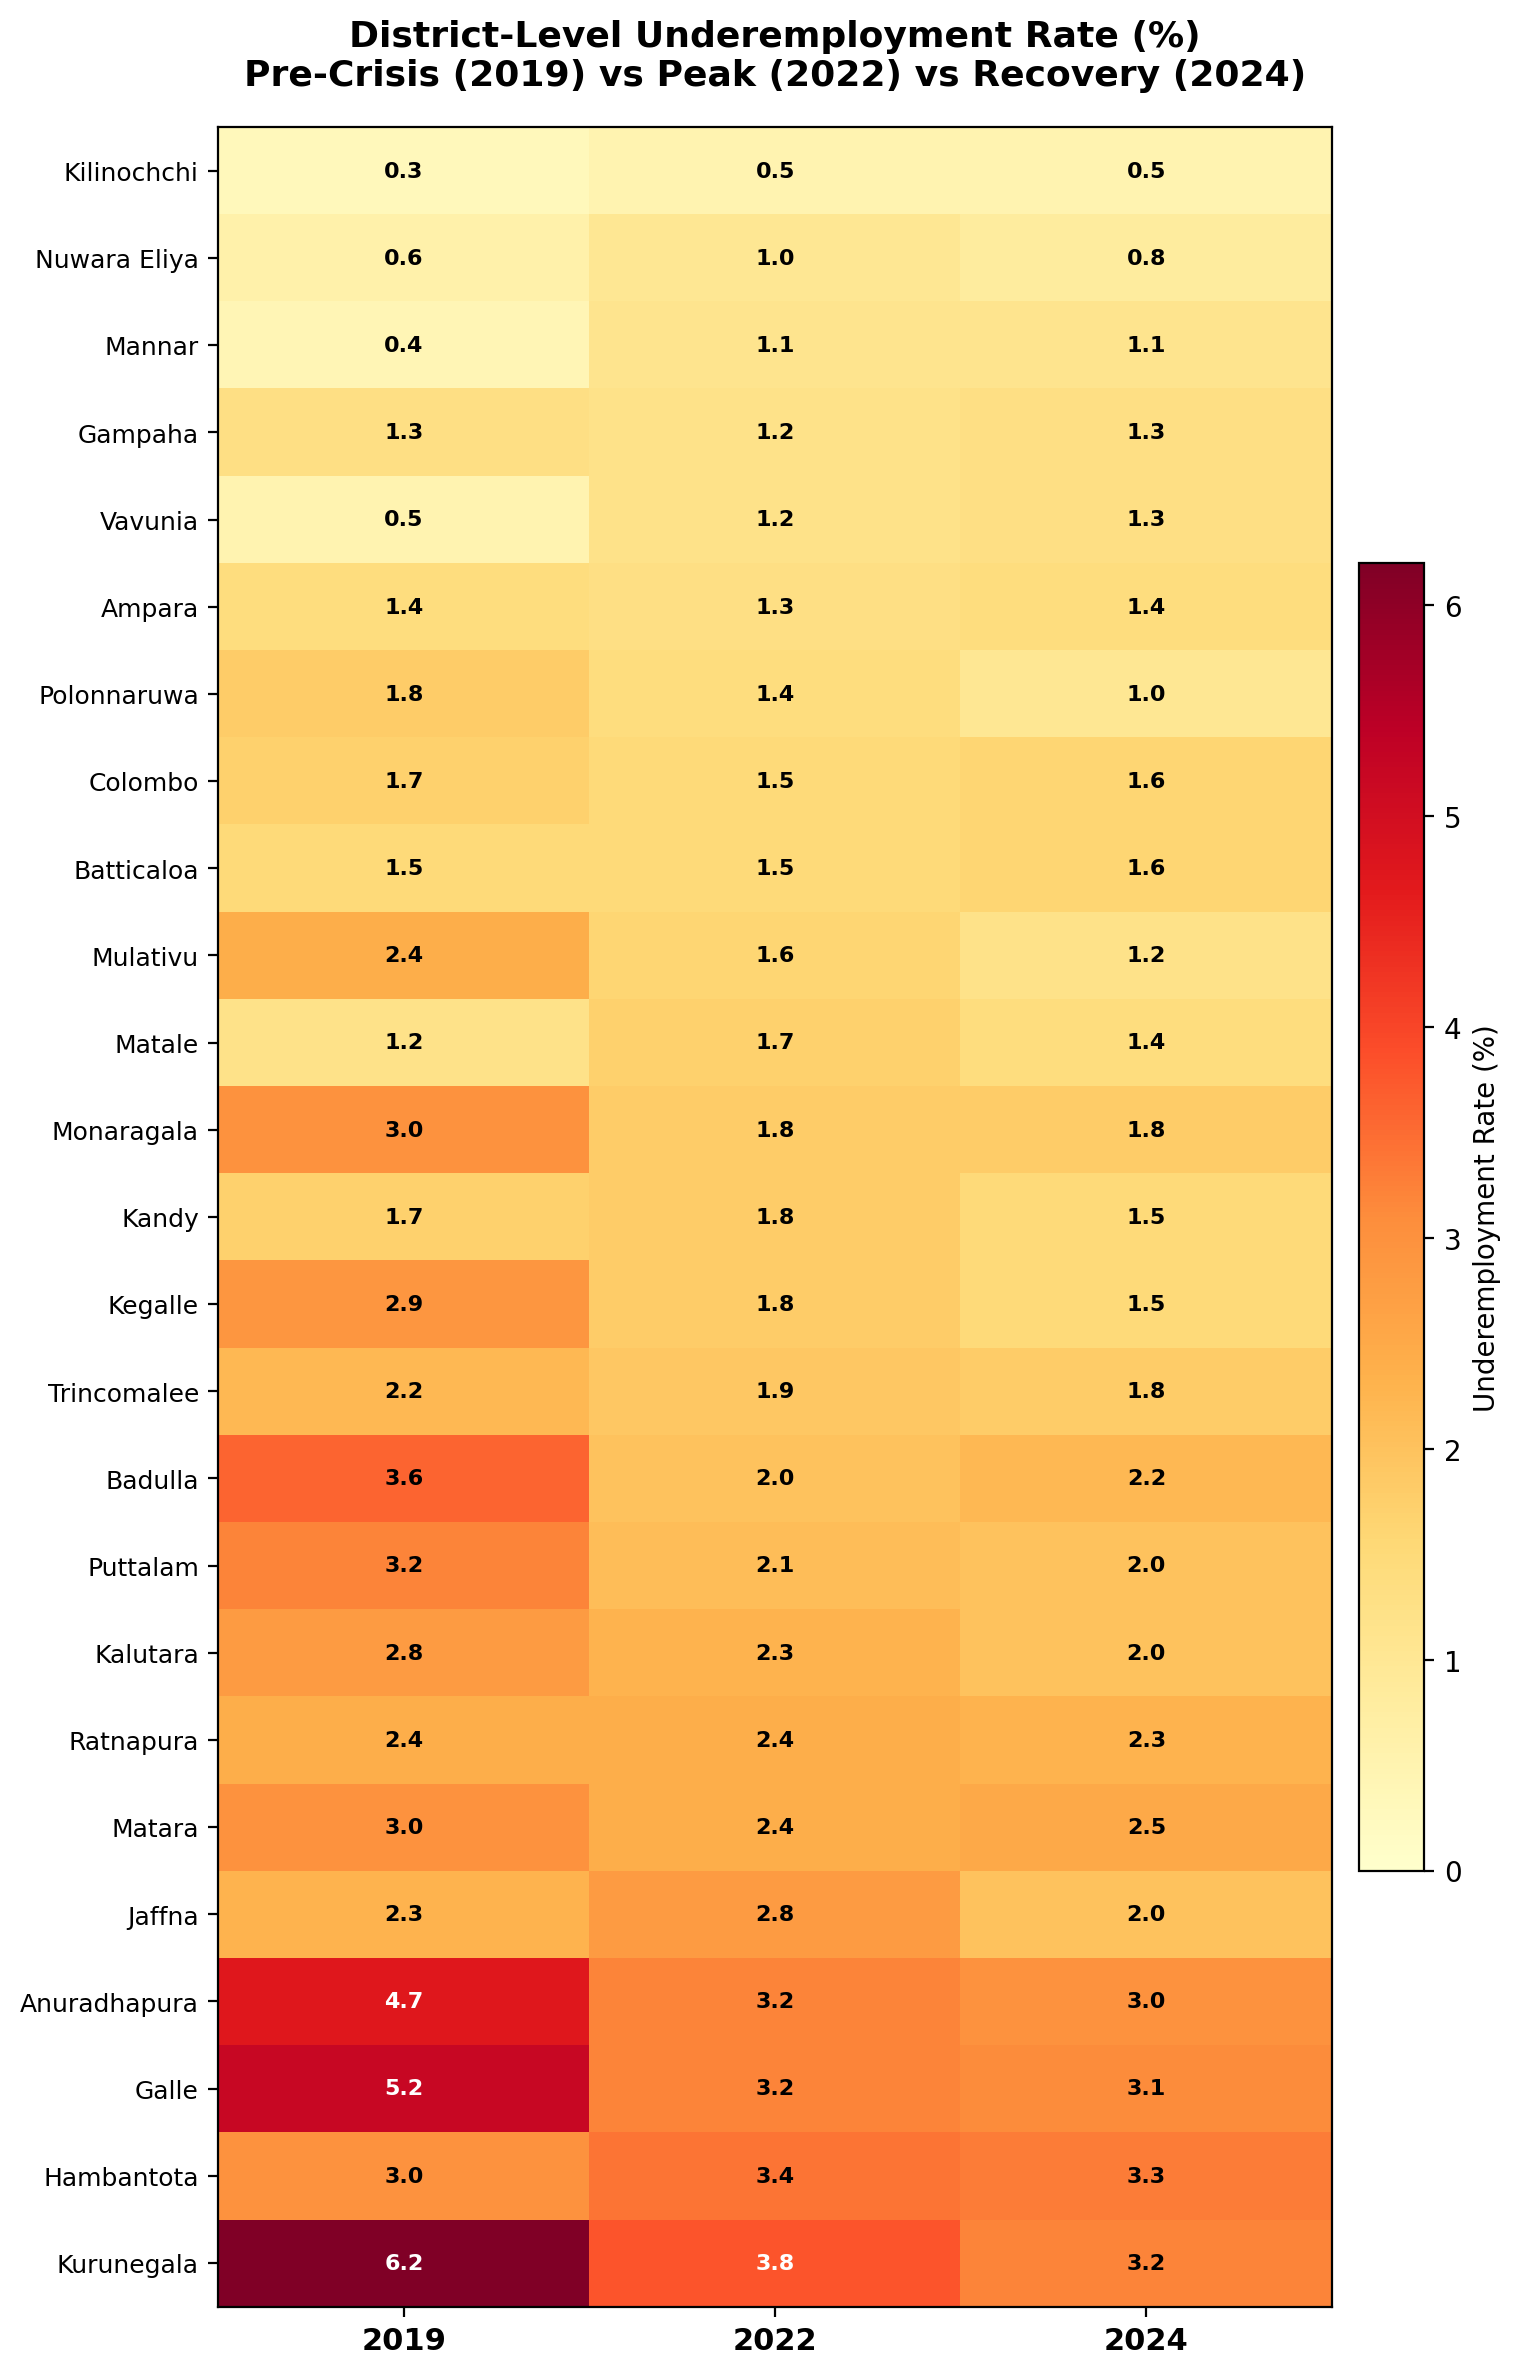
\includegraphics[width=0.98\columnwidth]{district_heatmap.png}
  \caption{District-level underemployment heatmap (25 districts,
    2019/2021/2022). Darker cells indicate higher underemployment.
    Northern and Southern districts show persistent hotspots.}
  \label{fig:district_heatmap}
\end{figure}

%% ===================================================
\section{Conclusion}
%% ===================================================

Quarterly LFS micro-data reveals crisis underemployment peaks of 32.6\%,
nine times the concurrent 3.8\% unemployment rate. Structural break tests
confirm 2021--2022 as a statistically significant rupture in the
underemployment--GDP--inflation system, with macro breaks leading the labour
market break by one year. The incorporated variables reveal two additional
findings: informal employment broke significantly in 2017, predating the
crisis and suggesting formalisation pressure as a structural precondition;
and part-time employment spiked in 2020 under COVID, acting as a precursor
to the 2022 hours-underemployment surge. SHAP (Eq.~\ref{eq:shap})
establishes GDP contraction and informal employment as the dominant drivers,
with Youth LFPR, remittances, and part-time employment capturing
complementary channels. The interaction model (Eq.~\ref{eq:interaction})
confirms structural amplification of GDP elasticity post-2022. ARDL bounds
testing on the quarterly dataset ($n{=}36$) resolves \textbf{RQ4}: the
Pesaran $F$-statistic of 7.25 confirms long-run cointegration at 1\%,
and the ECM speed-of-adjustment $\hat\lambda{=}{-}1.087$ ($p{=}0.003$)
indicates near-complete quarterly correction toward equilibrium. Long-run
GDP elasticity is $-0.39$~pp per 1~pp GDP growth. The sensitivity analysis
confirms SHAP rankings are strongly convergent across
hours-based and qualification-based definitions ($\rho = 0.893$,
$p = 0.007$). Gender-disaggregated analysis reveals distinct driver
structures: female underemployment is more inflation-sensitive while male
underemployment responds primarily to GDP contractions. The persistent
female--male gap ($W = 55.0$, $p = 0.001$) and widening qualification
gender gap (0.97~pp to 4.42~pp) indicate the crisis disproportionately
affected women's labour market outcomes. District-level analysis confirms
substantial spatial heterogeneity that informality alone does not explain.
Aggregate unemployment is an inadequate crisis barometer for Sri Lanka.

\textbf{Limitations.} The annual XGBoost model ($n{=}10$) achieves limited
out-of-sample fit; SHAP values are association measures, not causal
estimates. The 2022 LFS artefact complicates annual inference for the
hours-based series (mitigated by using the quarterly series for structural
tests). Johansen cointegration remains infeasible on annual data. The ECM
speed-of-adjustment $|\hat\lambda|{>}1$ indicates mild overshooting,
consistent with volatile crisis-period dynamics, and should be interpreted
with caution. Agricultural data ends at 2024; FAOSTAT 2025 crop indices
are not yet released. The gender Zivot-Andrews test lacks power at $n{=}10$;
quarterly gender data would strengthen break detection.

\textbf{Future work} will: (i) re-estimate ARDL/ECM on the expanded
quarterly dataset ($n{\approx}43$) once 2025~Q3--Q4 LFS data are released;
(ii) incorporate the 2025 annual LFS data; (iii) extend gender analysis to
quarterly disaggregation for higher-power break detection; and (iv) develop
district-level panel models to explain spatial heterogeneity beyond
informality.

\bibliographystyle{ACM-Reference-Format}
\bibliography{references}

\end{document}